\documentclass{article}

\usepackage{amsmath}
\usepackage{booktabs}
\usepackage{fullpage}
\usepackage{parskip}
\usepackage{tikz}
\usetikzlibrary{calc, shapes, patterns}

\begin{document}

\section*{\centering{Moran process}}
\subsection*{\centering{Fitness}}


\[
N=3
\text{ and }
A =
\begin{pmatrix}
    0 & 3 \\ 
    1 & 2
\end{pmatrix}
\]

\vspace{1cm}

\begin{center}
    \begin{tabular}{r|c|c}
        \toprule
                         & \(f(\text{Hawk})\)           & \(f(\text{Dove})\) \\
        \midrule
                         &                              & \\
        1 Hawk, 2 Doves  & \(0\times 0  + 3\times 2\)=6 & \phantom{\(0\times 0 + 3\times 2\)=6} \\
                         &                              & \\
        \midrule
                         &                              & \\
        2 Hawks, 1 Dove  &                              & \\
                         &                              & \\
        \bottomrule
    \end{tabular}
\end{center}

\subsection*{\centering{Probabilities}}

\begin{center}
    \begin{tabular}{r|r|c|c}
        \toprule
        & Select       & Selection: Birth   & Selection: Death   \\
        \midrule
        &             &                                                                          & \\
        &Hawk         & \(\frac{f(\text{Hawk})}{f(\text{Hawk}) + 2f(\text{Dove})}=\frac{6}{12}\) & \(\frac{1}{3}\)\\
        &             &                                                                          & \\
1 Hawk, 2 Doves        &             &                                                                          & \\
        &             &                                                                          & \\
        &Dove         &                                                                          & \\
        &             &                                                                          & \\
        \midrule
        &             &                                                                          & \\
        &Hawk         &                                                                          & \\
        &             &                                                                          & \\
2 Hawks, 1 Dove        &             &                                                                          & \\
        &             &                                                                          & \\
        &Dove         &                                                                          & \\
        &             &                                                                          & \\
        \bottomrule
    \end{tabular}
\end{center}

\newpage
\section*{\centering{Simulation}}

Use a D12 (12 sided dice) to simulate 1 Hawk taking over a population of Doves.

\begin{center}
   \begin{tabular}{r|c|c}
        \toprule
        State & Select Hawk values (birth) & Select Hawk values (death) \\
        \midrule
                        &                         &                         \\
        1 Hawk          & \(\{1, 2, 3, 4, 5, 6\}\)         & \(\{1, 2, 3, 4\}\)           \\
                        &                         &                         \\
        \midrule
                        &                         &                         \\
        2 Hawks         & \(\{1, 2, 3, 4, 5, 6, 8, 9\}\)         & \(\{1, 2, 3, 4, 6, 7, 8\}\)     \\
                        &                         &                         \\
        \bottomrule
    \end{tabular}
\end{center}


\subsection*{\centering{Example}}

\begin{center}
    \begin{tabular}{r|c|c|c}
        \toprule
        State & Birth: value rolled & Death: value rolled & Next state \\
        \midrule
                      &                   &                   &             \\
        1 Hawk        & 2                 & 1                 & 1 Hawk      \\
                      & (Select Hawk)     & (Select Hawk)     &             \\

                      &                   &                   &             \\
        1 Hawk        & 3                 & 5                 & 2 Hawks     \\
                      & (Select Hawk)     & (Select Dove)     &             \\

                      &                   &                   &             \\
        2 Hawks       & 10                 & 2                 & 1 Hawk      \\
                      & (Select Dove)     & (Select Hawk)     &             \\

                      &                   &                   &             \\
        1 Hawk        & 9                 & 1                 & \framebox{0 Hawks} \\
                      & (Select Dove)     & (Select Hawk)     &             \\
        \bottomrule
    \end{tabular}
\end{center}

\subsection*{\centering{Activity}}

Every time you arrive at 0 \textbf{or} 3 Hawks:

\begin{enumerate}
    \item Stop;
    \item Circle your final state
    \item Draw a line in the table (next page);
    \item Start again.
\end{enumerate}

\newpage

\begin{center}
    \begin{tabular}{r|c|c|c}
        \toprule
        Current state & Birth: value rolled & Death: value rolled & Next state \\
        \midrule
        1 Hawk        &                    &                     &            \\
                      &                    &                     &            \\
                      &                    &                     &            \\
                      &                    &                     &            \\
                      &                    &                     &            \\
                      &                    &                     &            \\
                      &                    &                     &            \\
                      &                    &                     &            \\
                      &                    &                     &            \\
                      &                    &                     &            \\
                      &                    &                     &            \\
                      &                    &                     &            \\
                      &                    &                     &            \\
                      &                    &                     &            \\
                      &                    &                     &            \\
                      &                    &                     &            \\
                      &                    &                     &            \\
                      &                    &                     &            \\
                      &                    &                     &            \\
                      &                    &                     &            \\
                      &                    &                     &            \\
                      &                    &                     &            \\
                      &                    &                     &            \\
                      &                    &                     &            \\
                      &                    &                     &            \\
                      &                    &                     &            \\
                      &                    &                     &            \\
                      &                    &                     &            \\
                      &                    &                     &            \\
                      &                    &                     &            \\
                      &                    &                     &            \\
                      &                    &                     &            \\
                      &                    &                     &            \\
                      &                    &                     &            \\
                      &                    &                     &            \\
                      &                    &                     &            \\
                      &                    &                     &            \\
                      &                    &                     &            \\
                      &                    &                     &            \\
                      &                    &                     &            \\
                      &                    &                     &            \\
                      &                    &                     &            \\
                      &                    &                     &            \\
                      &                    &                     &            \\
                      &                    &                     &            \\
                      &                    &                     &            \\
        \bottomrule
    \end{tabular}
\end{center}


\section*{\centering{Computation}}

\begin{center}
    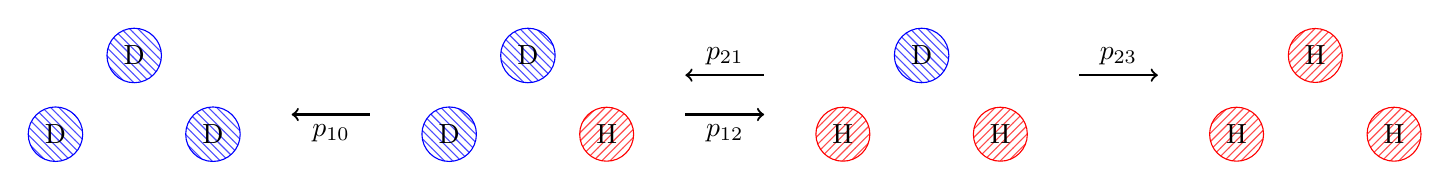
\begin{tikzpicture}[
        dove/.style={circle, pattern=north west lines, pattern color=blue!70, draw=blue},
        hawk/.style={circle, pattern=north east lines, pattern color=red!70, draw=red},
        ]

	\node (N1) at (1, 1) [dove] {D};
	\node (N2) at (0, 0) [dove] {D};
	\node (N3) at (2, 0) [dove] {D};

    \draw [thick, <-] ($(N1)!0.5!(N2) + (2.5, -.25)$) -- node [below] {\(p_{10}\)} ++(1, 0);

    \node (N1) at ($(N1) + (5, 0)$) [dove] {D};
    \node (N2) at ($(N2) + (5, 0)$) [dove] {D};
    \node (N3) at ($(N3) + (5, 0)$) [hawk] {H};

    \draw [thick, ->] ($(N1)!0.5!(N2) + (2.5, -.25)$) -- node [below] {\(p_{12}\)} ++(1, 0);
    \draw [thick, <-] ($(N1)!0.5!(N2) + (2.5, .25)$) -- node [above] {\(p_{21}\)} ++(1, 0);

    \node (N1) at ($(N1) + (5, 0)$) [dove] {D};
    \node (N2) at ($(N2) + (5, 0)$) [hawk] {H};
    \node (N3) at ($(N3) + (5, 0)$) [hawk] {H};

    \draw [thick, ->] ($(N1)!0.5!(N2) + (2.5, .25)$) -- node [above] {\(p_{23}\)} ++(1, 0);

    \node (N1) at ($(N1) + (5, 0)$) [hawk] {H};
    \node (N2) at ($(N2) + (5, 0)$) [hawk] {H};
    \node (N3) at ($(N3) + (5, 0)$) [hawk] {H};
    \end{tikzpicture}
\end{center}

\vspace{1cm}

Which gives:

\[
    p_{10}=\frac{6}{12}\frac{1}{3}=\frac{1}{6}\qquad
    p_{12}=\phantom{\frac{6}{12}\frac{2}{3}=\frac{1}{3}}\qquad
    p_{21}=\phantom{\frac{2}{8}\frac{2}{3}=\frac{1}{6}}\qquad
    p_{23}=\phantom{\frac{6}{8}\frac{1}{3}=\frac{1}{4}}
\]


\end{document}

